\documentclass[a4paper]{article}
\usepackage[utf8]{inputenc}
\usepackage{amsmath}
\usepackage{minted}
\usepackage{graphicx}
\usepackage{geometry}
\usepackage{floatrow}
\usepackage{layout}
\usepackage{amssymb}
\usepackage{multirow}
\usepackage{caption}
\usepackage{listings}
\geometry{margin=1in}
\usepackage{authblk}
\usepackage{indentfirst}
\usepackage{hyperref}
\hypersetup{
    colorlinks=true,
    linkcolor=blue,
    bookmarks=true,
    }

\begin{document}
\title{\textbf{\huge{Phase 1 Report}}}
\author{\textbf\large{Xining Li, Yi Zhao, Xiaoyan Liu, Yaguang Chen}}
\affil{\textbf{GaTech}}
\date{\today}
\maketitle
\begin{abstract}
This is abstract
\end{abstract}\maketitle
%	\tableofcontents
%%	Main	body	starts	here
%	Description	of	Section	1
\section{Table of Contents}

\begin{itemize}
	\item Inge's Animal Haven Data Types
	\begin{itemize}
		\item \hyperlink{data_types}{Data Types}
	\end{itemize}
\end{itemize}

\begin{itemize}
	\item Inge's Animal Haven Constraints
	\begin{itemize}
		\item \hyperlink{business_logic_cons}{Business Logic Constraints}
	\end{itemize}
\end{itemize}

\begin{itemize}
	\item Task Decomposition with Abstract Code:
	\begin{itemize}
		\item \hyperlink{login}{Login}
		\item \hyperlink{animal_dashboard}{Animal Dashboard}
		\item \hyperlink{add_animal}{Add Animal}
		\item \hyperlink{animal_detail}{Animal Detail}
		\item \hyperlink{vaccinations}{Vaccinations}
		\item \hyperlink{adoption}{Adoption}
		\item \hyperlink{add_adoption_app}{Add Adoption Application}
		\item \hyperlink{adoption_app_review}{Adoption Application Review}
		\item \hyperlink{animal_control_report}{Animal Control Report}
		\item \hyperlink{volunteer_of_the_month}{Volunteer of the Month}
		\item \hyperlink{monthly_adoption_report}{Monthly Adoption Report}
		\item \hyperlink{volunteer_lookup}{Volunteer Lookup}
		\item \hyperlink{vaccine_reminder_report}{Vaccine Reminder Report}
	\end{itemize}

\end{itemize}

\pagebreak

\hypertarget{data_types}{\section{Data Types}}

\begin{table}[H]
		\centering
	\begin{tabular}{|l|l|l|}
		Attribute     & Data Type & is Nullable \\
		User Name     & String    & Not Null \\
		Password      & String    & Not Null \\
		email address & String    & Not Null \\
		First Name    & String    & Nullable \\
		Last Name     & String    & Nullable
	\end{tabular}
\caption{User}
\end{table}



\begin{table}[H]
	\centering
	\begin{tabular}{|l|l|l|}
		Attribute     & Data Type & is Nullable \\
		Number of Hours per day     & Integer    & Not Null \\
		Password      & String    & Not Null \\
	\end{tabular}
	\caption{Volunteer}
\end{table}



\begin{table}[H]
	\centering
	\begin{tabular}{|l|l|l|}
		Attribute     & Data Type & is Nullable \\
		Pet id     & String    & Not Null \\
		Name      & String    & Not Null \\
		Microchip Ids      & String    & Nullable \\
		Surrender date      & Integer    & Not Null \\
		Surrender Reason      & String    & Nullable \\
		Species      & String    & Nullable \\
		Breed      & List[String]    & Nullable \\
		Sex      & String   & Not Null \\
		Age      & Integer   & Nullable \\
		Alteration Status      & String   & Not Null \\
	\end{tabular}
	\caption{Animal}
\end{table}

\begin{table}[H]
	\centering
	\begin{tabular}{|l|l|l|}
		Attribute     & Data Type & is Nullable \\
		Application Number     & Integer & Not Null \\
		Phone Number     & Long & is Nullable \\
		Email Address     & String & is Nullable \\
		Address\_Street    & String & is Nullable \\
		Address\_City   & String & is Nullable \\
		Address\_State   & String & is Nullable \\
		Address\_ZipCode  & String & is Nullable \\
		Applicant Name  & String & Not Null \\
		Co-Applicant Name  & String & is Nullable \\
	\end{tabular}
	\caption{Contact Information}
\end{table}

\begin{table}[H]
	\centering
	\begin{tabular}{|l|l|l|}
		Attribute     & Data Type & is Nullable \\
		Associated Animal     & String & Not Null \\
		Associated Application     & Integer & Not Nullullable \\
		Adoption Date     & Integer & Not Null \\
		Adoption Fee     & Integer & Not Null \\
	\end{tabular}
	\caption{Adoption Information}
\end{table}

\begin{table}[H]
	\centering
	\begin{tabular}{|l|l|l|}
		Attribute     & Data Type & is Nullable \\
		Associated Species     & String & Not Null \\
		Vaccination Type   & String & Not Null \\
		Required     & Boolean & Not Null \\
	\end{tabular}
	\caption{Vaccination Requirement}
\end{table}

\begin{table}[H]
	\centering
	\begin{tabular}{|l|l|l|}
		Attribute     & Data Type & is Nullable \\
		Associated Animal     & String & Not Null \\
		Vaccination Type   & String & Not Null \\
		Expiration Date     & Integer & Not Null \\
		Vaccination Number    & String & Not Null \\
		Entrance person    & String & Not Null \\

	\end{tabular}
	\caption{Vaccination Administration Table}
\end{table}

\pagebreak

\hypertarget{business_logic_cons}{\section{Business Logic Constraints}}

\subsection*{User}

\begin{itemize}
	\item Inge will choose each member of Users and decide the size of Users.
	\item New Users can only be added by the database adminstrator with Igne's approval.
	\item Users' information will be maintained by the database adminstrator.
\end{itemize}

\subsection*{Animals}

\begin{itemize}
	\item Can only store information of 30 cats and 15 dogs. Limit is adjustable as needed or as the shelter expands.
\end{itemize}

\subsection*{Monthly Adoption Report}
\begin{itemize}
	\item  A single adoption application can only be matched to a single animal
	\item  animal with multiple breeds combined into a single value in alphabetical order
	\item  A single adoption application can only be matched to a single animal

\end{itemize}

\subsection*{Vaccine Reminder Report}
\begin{itemize}

    \item The system should not allow you to enter a vaccine that is not yet due for an animal or that they have already been given.
    \item Animal breeds combined to one
    \item Vaccination could be updated by dba
    \item Sort the data in the ascending order of the vaccination due date (most recent date to latest date) and by pet ID ascending.

\end{itemize}

\pagebreak
\section{Task Decomposition with Abstract Code}

\hypertarget{login}{\subsection{Login}}
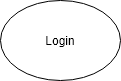
\includegraphics[scale = 0.6]{login.png}

\begin{itemize}
	\item Lock Type: Read-only on the \textbf{User} table
	\item Number of Locks: Semaphore permits depend on the server and database power. In our case, we should choose 10.
	\item Enabling Condition: None
	\item Frequency: Around 200 logins per day
	\item Consistency(ACID): Not critical, order is not critical
	\item Substacks: Mother Task is not needed. No decomposition is needed.
\end{itemize}

\subsubsection*{Abstract Code}

\begin{itemize}
        \item User enters \textbf{email}, \textbf{password} input fields.
        \item If data validation is successful for both username and password input fields, then:

\item When \textit{Enter} button is clicked \begin{itemize}
        \item If User record is found and user entered password match the username's key associated password in the \textbf{User} table: Store login information as session variable '\$UserID', and go to the \underline{\textbf{Animal Dashboard}}
	\item Else: Go back to the \underline{\textbf{Login}}
	\end{itemize}
\end{itemize}

\hypertarget{animal_dashboard}{\subsection{Animal Dashboard}}
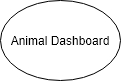
\includegraphics[scale = 0.6]{animal_dashboard.png}

\begin{itemize}
        \item Lock Type: Lookup \textbf{Animal} Name, Species, Breed, Sex, Alteration Status, Age, and Adoptability Status. Read-only on the \textbf{Animal} table
        \item Number of Locks: Semaphore permits depend on the server and database power. In our case, we should choose 10.
	\item Enabling Condition: Trigger by successful login
        \item Frequency: As same as the login
        \item Consistency(ACID): Not critical, order is not critical
        \item Substacks: Mother Task is not needed. No decomposition is needed.
\end{itemize}

\subsubsection*{Abstract Code}

\begin{itemize}
	\item Show the animal’s name, species, breed, sex, alteration status, age, and adoptability status by the result of the corresponding SQL query.
	\item Populate species and adoptability status dropdowns, if no buttons are pushed, do nothing. If clicking on sepcies and/or adopatability status, query corresponding animals and display them on dashboard only.

	\item Upon: \begin{itemize}
		\item Clicking on each column would pop out 2 choices: sort in increasing order, sort in decreasing order.
		\item Clicking on the animal's name will go to the \underline{\textbf{Animal Detail}}'s Servlet (implemented using RestFul API GET method).
	\end{itemize}
	\item Show the number of available spaces.
	\item if the user has appropriate permission (fetched by the corresponding SQL query), an \textit{Add Animal} button will show directing to the \underline{\textbf{Add Animal}} screen.
        \item if the user has appropriate permission (fetch by the corresponding SQL query), an \textit{Add Adoption Application} button will show directing to the \underline{\textbf{Add Adoption Application}} screen.
\end{itemize}

\hypertarget{add_animal}{\subsection{Add Animal}}
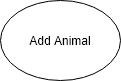
\includegraphics[scale = 0.6]{add_animal.png}

\begin{itemize}
	\item Lock Type: Lock on on the process of the successfully converted data structure from the post request sending the \textit{Add Animal} process in the database.
	\item Number of Locks: Single Lock
	\item Enabling condition: Trigger by the previous \underline{\textbf{Animal Dashboard}}'s \textit{Add Animal} Button.
	\item Frequency: Low, about 5 per day.
	\item Consistency (ACID): Super critical.
	\item Substacks: Mother task is not needed.
\end{itemize}

\subsection*{Abstract Code}

\begin{itemize}
	\item Process user's post request and convert to a data structure (for example Json or POJO)
	\item Validate user input, if valid continue, else return user the error message.
	\item Acquire permit from the semaphore
	\item TRY:
	\begin{itemize}

	\item Parse the animal's species from the user's post request
	\item If the animal's species from the user's post request is exist in the database and the number of availability associated with the animal's species is greater than 0:
		\begin{itemize}
			\item Generate the unique petId by accessing the \textbf{Animal} table and pass to the setter of the petId field of the upper-mentioned data structure.
			\item Submit the data structure to the database.
			\item Take the user to the \underline{\textbf{Animal Detail}} Screen.
		\end{itemize}
	\item Elae:
		\begin{itemize}
			\item Return the user an error message with the corresponding error code.
		\end{itemize}

	\end{itemize}
	\item Catch Exception:
		\begin{itemize}
		\item Log the error message and return the error message to the user.
		\end{itemize}
	\item Finally:
		\begin{itemize}
		\item Rlease the permit to the semaphore.
		\end{itemize}
\end{itemize}


\hypertarget{animal_detail}{\subsection{Animal Detail}}
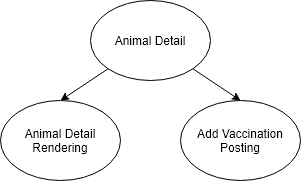
\includegraphics[scale = 0.6]{animal_detail.png}

\begin{itemize}
	\item Lock Type: Synchronized lock on the animal's hashcode. Lookups of \textbf{Animal} information from  and \textbf{Vaccinations} information from \textbf{Animal} table.
	\item Number of Locks: Lock on the AddVaccinationServlet's get and post methods
	\item Enabling condition: Trigger by the previous \underline{\textbf{Animal Dashboard}}'s \textit{Animal's name} Button.
	\item Frequency: Medium, about 50 per day.
	\item Consistency (ACID): Not critical.
	\item Substacks: Mother task is not needed. Two substacks:
	\item   \begin{itemize}
				\item Animal Detail rendering
				\item Add Vaccination Posting
			\end{itemize}
\end{itemize}


\begin{itemize}
	\item Show animal's all details (attributes) by the result of the corresponding SQL query.
	\item Show a "Vaccinations" section which shows any Vaccination history.
	\item Show \textit{Add Vaccination} button if the corresponding animal has not been adopted.
	\item Show \textit {Adopt pet} button if the animal is eligible for adoption and if the session user has the permission.
\end{itemize}

\subsection*{Abstract Code}

\subsubsection*{AnimalDetailServlet}

Background: Animal Dashboard's restful API takes the user to the corresponding Animal Detail's front end, and the Animal Detail's front end call the AnimalDetailServlet using the GET method.

And here is the implementation of the AnimalDetailServlet's get method.
\begin{itemize}
	\item the AnimalDetailServlet query the database with the restful api's parameter (\textbf{PetId}) and convert to a POJO
	\item the AnimalDetailServlet return the Json converted from the POJO to the front end.
	\item the AnimalDetailServlet call the AddVaccinationServlet using the GET method and return the user the vaccination that can be implemented.
	\item (frontend code) the user can optionally call the AddVaccinationServlet using the POST method.
\end{itemize}


\subsubsection*{AddVaccinationServlet}

Background: Animal Dashboard's restful API takes the user to the corresponding Animal Detail's front end, and the Animal Detail's front end call the AddVaccinationServlet using the GET method.


\begin{lstlisting}
	public class Vaccination {
		@NotNull Enum VaccinationType;
		@NotNull Date date;
		@NotNull Date nextDoseDate;
		Long vaccineTagNumber;
	}


	public class AddVaccinationServlet extends HttpServlet {
		public final Semaphore vaccinationSemaphore= new Semaphore(1);
		Set<VaccinationType> Get(Animal animal){
			synchronized (animal.getSingleton()){
				if (!animal.eligibleForAdoption()){
				return null;
				} else {
					return animal
						.getSpecies()
						.getRequiredVaccinations()
						.setSubtraction(animal
							.implementedVaccinations
						);
				}
			}
		}
		void Post(Set<Vaccination> userImplementations) {
			synchronized (animal.getSingleton()){
				vaccinationSemaphore.acquire();
				for (Vaccination v: userImplementations) {
					/*
					implementVaccination talks to
					the database and put the corresponding
					vaccination into the animal's
					corresponding vaccination table.
					*/
					DataBaseSingleton.get(animal)
					.implementVaccination(v);
				}
				vaccinationSemaphore.release();
			}
		}
	}
\end{lstlisting}


\hypertarget{vaccinations}{\subsection{Vaccinations}}
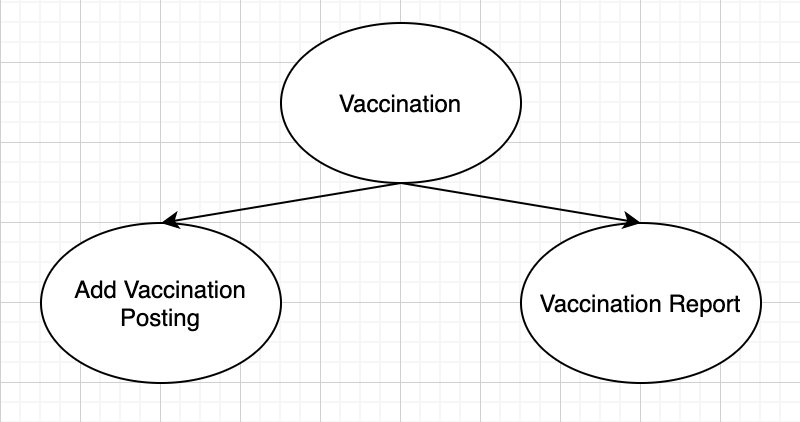
\includegraphics[scale = 0.6]{vaccination.png}

\begin{itemize}
	\item Lock Type: Look up the \textbf{Vaccinations} table.
	\item Number of Locks: Single Lock
	\item Enabling condition: Trigger by the previous \underline{\textbf{Animal Detail}}'s \textit{Add Vaccinations} Button.
	\item Frequency: Different Frequencies
	\item Consistency (ACID): Not critical
	\item Substasks: Mother task is the \underline{\textbf{Animal Detail}}.
\end{itemize}

\subsubsection*{Abstract Code}

\begin{itemize}
	\item Populate vaccinations dropdown lists
	\item When submit button is not clicked, nothing happened
	\item When submit button is clicked:
	\begin{itemize}
	    \item If vaccine is not chosen: catch Exception, log error message and return the error message to the user;
	    \item If vaccine is chosen, not both vaccination date or next does date are entered: catch Exception, log error message to the user;
	    \item  Else: update Animal table,
	 \end{itemize}
	 \item If submit successfully, Display \underline{\textbf{Animal Detail}}
\end{itemize}

\hypertarget{adoption}{\subsection{Adoption}}
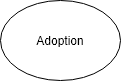
\includegraphics[scale = 0.6]{adoption.png}

\begin{itemize}
	\item Lock Type: Look up Adopter Contact Information table, and is read-only. Lookup Adoption Information  table, can read, update, insert
	\item Number of Locks: Single Lock
	\item Enabling condition: Trigger by the previous \underline{\textbf{Animal Detail}}'s \textit{Add Adoption} Button.
	\item Frequency: Different Frequencies
	\item Consistency (ACID): Not critical
	\item Substasks: Mother Task is not needed. No decomposition is needed.
\end{itemize}

\subsubsection*{Abstract Code}

\begin{itemize}
	\item Show search dialog where user can search both applicant's last name and co-applicant's last name
	\item Query and display Applicant's contact information
	\item If select Adopter, show pop up for adoption date and adoption fee
	\item If enter adoption date and adoption fee, update \textbf{Adoption Information}  table, display  \underline{\textbf{Animal Detail}}
	\item If cancellation, display  \underline{\textbf{Animal Detail}}
\end{itemize}


\hypertarget{add_adoption_app}{\subsection{Add Adoption Application}}
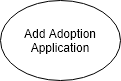
\includegraphics[scale = 0.6]{add_adoption_app.png}

\begin{itemize}
	\item Lock Type: Look up Adopter \textbf{Contact Information} table
	\item Number of Locks: Single Lock
	\item Enabling condition: Trigger by the previous \underline{\textbf{Animal Dashboard}}'s \textit{Add Adoption Application} Button.
	\item Frequency: Different Frequencies
	\item Consistency (ACID): Not critical
	\item Substasks:  Mother Task is not needed. No decomposition is needed.
\end{itemize}

\subsubsection*{Abstract Code}

\begin{itemize}
	\item Show screen to let users enter applicant information including Application first name and last name, Address (street, city, state, zip code), phone number, email address, Date of Application, (optional) co-applicant first name and last name
	\item When click submit button:
	\begin{itemize}
	    \item If at least one contact information is not entered: catch Exception, log error message and return the error message to the user;
	    \item Else: Add \textbf{Contact Information}, display application ID generated by system
	\end{itemize}
	\item When submit button is not clicked, nothing happen

\end{itemize}



\hypertarget{adoption_app_review}{\subsection{Adoption Application Review}}
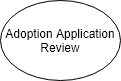
\includegraphics[scale = 0.6]{adoption_app_review.png}

\begin{itemize}
	\item Lock Type: Look up Contact Information table
	\item Number of Locks: Single Lock
	\item Enabling condition: Trigger by the login by Inge and her \underline{\textbf{Animal Dashboard}}
	\item Frequency: Low Frequency
	\item Consistency (ACID): Not critical
	\item Substasks:  Mother Task is not needed. No decomposition is needed.
\end{itemize}

\subsubsection*{Abstract Code}

\begin{itemize}
	\item Find applicationID with pending approval, display applicationID and status
	\item Update status with dropdown, approved or rejected, Save application status to Contact Information table


\end{itemize}




\hypertarget{animal_control_report}{\subsection{Animal Control Report}}
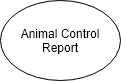
\includegraphics[scale = 0.6]{animal_control_report.png}

\begin{itemize}
	\item Lock Type: Read-only lookup of the numbers of animals surrendered by Animal Control in a month and each animal's information from Animal table. Another read-only lookup of count and information of current-month adopted animals which were in the rescue for 60 or more days from Animal table and Adoption Informationl.
	\item Number of Locks: Several different schema constructs are needed.
	\item Enabling condition: Trigger by the previous \underline{\textbf{Animal Dashboard}}'s \textit{Animal Control Report} Button.
	\item Frequency: Low - Both have the same frequency
	\item Consistency (ACID): Not critical
	\item Substasks: Mohter task is not needed.
\end{itemize}

\subsubsection{Abstract Code}

\begin{itemize}
	\item SuperUser clicked on \textit{Animal Control Report} button from \underline{\textbf{Animal Dashboard}}:
	\item Run the \textbf{Animal Control Report} task: query for animals' information.
	\begin{itemize}
		\item Select month;
		\item Find the animals that was surrendered by Animal Control in selected month;
		\item Count these animals;
		\item Display the volume of this count;
		\item For each animal in this count:
		\begin{itemize}
			\item Sort by Pet ID ascending;
			\item Display animal's information;
		\end{itemize}
		\item Find the animals that was adopted in selected month;
		\item Find these adopted animal's adopted date and surrendered date;
		\item For each animal that was adopted in selected month:
		\begin{itemize}
			\item Calculate sheltered dates
			\item If sheltered dates are greater or equal to 60 days:
			\begin{itemize}
				\item Add this animal to count
			\end{itemize}
		\end{itemize}
		\item Display the volume of this count;
		\item For each animal in this count:
		\begin{itemize}
			\item Display animal's information.
		\end{itemize}
	\end{itemize}
\end{itemize}

\hypertarget{volunteer_of_the_month}{\subsection{Volunteer of the Month}}
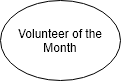
\includegraphics[scale = 0.6]{volunteer_of_the_month.png}

\begin{itemize}
	\item Lock Type: Read-only lookup of Personal information and total hours volunteered in a month for a VolunteerUser.
	\item Number of Locks: Single
	\item Enabling condition: Trigger by the previous \underline{\textbf{Animal Dashboard}}'s \textit{Volunteer of the Month} Button.
	\item Frequency: Low
	\item Consistency (ACID): Not critical
	\item Substasks: Mother Task is not needed. No decomposition is needed.
\end{itemize}

\subsubsection{Abstract Code}

\begin{itemize}
	\item SuperUser clicked on \textit{Volunteer of the Month} button from \underline{\textbf{Animal Dashboard}}:
	\item Run the \textbf{Volunteer of the Month} task: query for information and volunteered hours about the volunteers.
	\begin{itemize}
		\item Select month and year;
		\item Find all volunteers that has volunteered for selected month and year;
		\item Calculate the total volunteered hours for each of these volunteers;
		\item Sort the list of volunteers by descending total hours volunteered for selected month and year;
		\item Display first 5 volunteers' first name, last name, email address and total volunteered hours in that month
	\end{itemize}
\end{itemize}




\hypertarget{monthly_adoption_report}{\subsection{Monthly Adoption Report}}
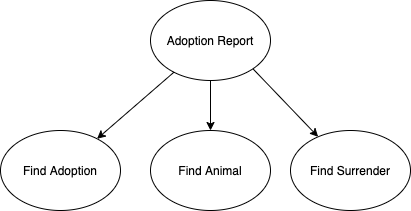
\includegraphics[scale = 0.6]{adoption_report.png}

\subsubsection*{Tasks decomposition}
\begin{itemize}
	\item Lock Type: All three read-only action
    \item Number of Locks: Three schemas: adoption, surrender and animal
    \item Enabling condition: All 3 enabled by link clicked in Inge's Animal Dashboard
    \item Frequency: Low-all 3 have similar frequency and table need monthly frequency
    \item Consistency (ACID): consistency is not critical
    \item Subtasks: all 3 must be done, mother task is needed. Should be decomposed to 3 different sub-tasks
    \begin{itemize}
        \item animal, surrender and adoptions
    \end{itemize}

\end{itemize}

\subsubsection*{Abstract Code}

\begin{itemize}
	\item \textbf{find the adoption} info for this month
	\item \textbf{find the surrender} info for this month
    \item \textbf{find the animal} info according to adoption and surrender
\item group by species, breed and count total
    \begin{itemize}
        \item  order by time and alphabetical order
        \item combine breed for mixed animal

    \end{itemize}




\end{itemize}




\hypertarget{volunteer_lookup}{\subsection{Volunteer Lookup}}
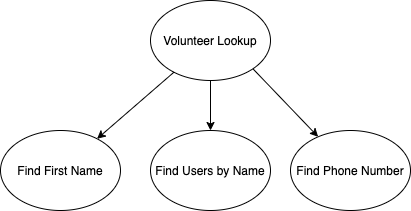
\includegraphics[scale = 0.6]{volunteer_lookup.png}

\subsubsection*{Constrains}
\begin{itemize}

    \item order by last name ascending and first name ascending.
\end{itemize}

\subsubsection*{Tasks decomposition}
\begin{itemize}
	\item  Lock types: Only two lookups to users and volunteer table is needed. read only action
    \item Number of Locks: two schema, users  and volunteer
    \item Enabling Conditions: all 2 enabled by link clicked in Inge's Animal Dashboard
    \item Frequency: volunteer frequency might be lower than user table, depends on how
    many volunteer vs employees
    \item Consistency (ACID): consistency is not critical
    \item Subtasks: could be decomposed to 2 sub-tasks
    \begin{itemize}

        \item find users by first and last name and email
        \item find phone number from volunteer table

    \end{itemize}

\end{itemize}
\subsubsection*{Abstract Code}

\begin{itemize}
	\item \textbf{find people} by their first name matching the search item (jon means jonson, jonstone etc.)
	\item \textbf{find users} by first and last name and email
    \item \textbf{find phone number} from volunteer table

    \item Data Validation
    \begin{itemize}

        \item - if user type in non-string type, it will be transform to string type
        \item - if user type noting in either first name or last name, transform into ''

    \end{itemize}

    \item SQL
    \begin{verbatim}
    SELECT l.first_name,
           l.last_name,
           v.phone_number,
           l.email_address
    FROM Volunteer v
      LEFT JOIN LoginUser l ON v.username = l.username
    WHERE l.first_name LIKE CONCAT('$First_Name','%')
    AND   l.last_name LIKE CONCAT('$Last_Name','%')
    ORDER BY l.last_name,
             l.first_name;
\end{verbatim}


\end{itemize}




\hypertarget{vaccine_reminder_report}{
\subsection{Vaccine Reminder Report }}
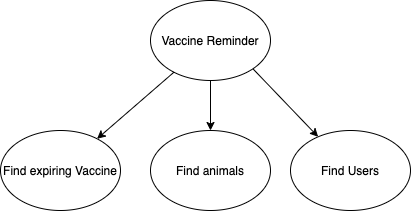
\includegraphics[scale = 0.6]{vaccine_reminder.png}

\subsubsection*{Tasks decomposition}
\begin{itemize}
	\item Lock Types: All 3 read-only lookups options.
	\item 3 tables: user, vaccination, animal
    \item Enabling Conditions: all 3 enabled by link clicked in Inge's Animal Dashboard
    \item Consistencyt (ACID): consistency is important, when user is updating animal, this report should be unavailable
    \item Frequency: frequency are similar, consistency is not important
 %   \item Vaccine enabled by employee only when  surrendered
    \item Subtasks: all 3 must be done, mother task is needed. Should be decomposed to 3 different sub-tasks

    \begin{itemize}

        \item animal, surrender and vaccination


    \end{itemize}

\end{itemize}
\subsubsection*{Abstract Code}

\begin{itemize}
	\item User expiration date to \textbf{find all vaccine} that are expiring
    \item \textbf{Find animals} by vaccine activity id
    \item \textbf{Find person} who did the vaccine

Here is the detailed code

\subsubsection*{VaccineReminderReportServlet}

Background: Animal Dashboard's restful API takes the user to the corresponding Animal Detail's front end, and the Animal Detail's front end call the AddVaccinationServlet using the GET method.


\begin{lstlisting}
	public class VaccineReminderReportServlet extends HttpServlet {

		public JsonObject getVaccineReminderReport(Time t){
			AddVaccinationServlet.vaccinationSemaphore.acquire();

			Result result = VaccineReminderReport
				.getInstnace()
				.getSqlSession()
				.query(t);

			AddVaccinationServlet.vaccinationSemaphore.release();
			return result.toJson();

		}

	}
\end{lstlisting}

\end{itemize}

\end{document}
